\begin{figure}[t]
\centering
\resizebox{0.97\linewidth}{!}{%
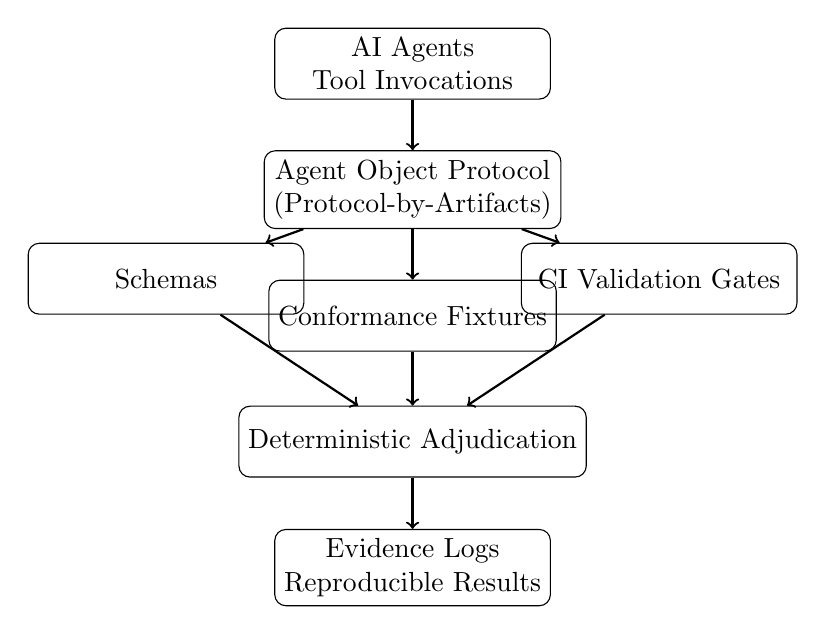
\begin{tikzpicture}[
node distance=1.6cm,
box/.style={draw, rounded corners, align=center, minimum width=3.5cm, minimum height=0.9cm},
arrow/.style={->, thick}
]

\node[box] (agents) {AI Agents \\ Tool Invocations};

\node[box, below of=agents] (protocol) {Agent Object Protocol \\ (Protocol-by-Artifacts)};

\node[box, below left of=protocol, xshift=-2cm] (schema) {Schemas};
\node[box, below of=protocol] (fixtures) {Conformance Fixtures};
\node[box, below right of=protocol, xshift=2cm] (gates) {CI Validation Gates};

\node[box, below of=fixtures] (adjudication) {Deterministic Adjudication};

\node[box, below of=adjudication] (evidence) {Evidence Logs \\ Reproducible Results};

\draw[arrow] (agents) -- (protocol);

\draw[arrow] (protocol) -- (schema);
\draw[arrow] (protocol) -- (fixtures);
\draw[arrow] (protocol) -- (gates);

\draw[arrow] (schema) -- (adjudication);
\draw[arrow] (fixtures) -- (adjudication);
\draw[arrow] (gates) -- (adjudication);

\draw[arrow] (adjudication) -- (evidence);

\end{tikzpicture}
}

\caption{Architecture of the Agent Object Protocol (AOP). Protocol specifications are transformed into executable artifacts (schemas, fixtures, and CI validation gates) enabling deterministic adjudication of AI agent artifacts.}

\label{fig:aop_architecture}
\end{figure}
